\documentclass[10pt]{extarticle}
\title{}
\author{Avinash Iyer}
\date{}
\usepackage[shortlabels]{enumitem}

%font setup
%
\usepackage{newpxtext,eulerpx}
\usepackage[T1]{fontenc}
\usepackage[utf8]{inputenc}

%paper setup
\usepackage{geometry}
\geometry{letterpaper, portrait, margin=1in}
\usepackage{fancyhdr}
\usepackage{soul}

%symbols
\usepackage{amsmath}
\usepackage{mathtools}
\usepackage{amssymb}
\usepackage{hyperref}
\usepackage{gensymb}


%chemistry stuff
\usepackage[version=4]{mhchem}
\usepackage{chemfig}

%plotting
\usepackage{pgfplots}
\usepackage{tikz}
\tikzset{middleweight/.style={pos = 0.5, fill=white}}
\tikzset{weight/.style={pos = 0.5, fill = white}}
\tikzset{lateweight/.style={pos = 0.75, fill = white}}
\tikzset{earlyweight/.style={pos = 0.25, fill=white}}

%\usepackage{natbib}

%graphics stuff
\usepackage{graphicx}
\graphicspath{ {./images/} }

%code stuff
%when using minted, make sure to add the -shell-escape flag
%you can use lstlisting if you don't want to use minted
%\usepackage{minted}
%\usemintedstyle{pastie}
%\newminted[javacode]{java}{frame=lines,framesep=2mm,linenos=true,fontsize=\footnotesize,tabsize=3,autogobble,}
%\newminted[cppcode]{cpp}{frame=lines,framesep=2mm,linenos=true,fontsize=\footnotesize,tabsize=3,autogobble,}

\usepackage{listings}
\usepackage{color}
\definecolor{dkgreen}{rgb}{0,0.6,0}
\definecolor{gray}{rgb}{0.5,0.5,0.5}
\definecolor{mauve}{rgb}{0.58,0,0.82}

\lstset{frame=tb,
	language=Java,
	aboveskip=3mm,
	belowskip=3mm,
	showstringspaces=false,
	columns=flexible,
	basicstyle={\small\ttfamily},
	numbers=none,
	numberstyle=\tiny\color{gray},
	keywordstyle=\color{blue},
	commentstyle=\color{dkgreen},
	stringstyle=\color{mauve},
	breaklines=true,
	breakatwhitespace=true,
	tabsize=3
}
% text + color boxes
\usepackage{tcolorbox}
\tcbuselibrary{breakable}
\newtcolorbox{problem}[1]{colback = white, title = {#1}, breakable}
\newtcolorbox{solution}{colback = white, colframe = black!75!white, title = Solution, breakable}
%including PDFs
\usepackage{pdfpages}
\setlength{\parindent}{0pt}

\pagestyle{fancy}
\fancyhf{}
\rhead{Avinash Iyer}
\lhead{Class Notes}
\begin{document}
  \section*{2.3}%
  \begin{problem}{Definition}
    A \textbf{weighted graph} $G$ is a graph alongside a function $w: E(G) \rightarrow \mathbb{R}^+$.\\

    If $G$ is a weighted graph and $H\subseteq G$, then, $w(H):=\sum\limits_{e\in E(H)} w(e)$.\\

    A \textbf{minimum weight spanning tree} (or MWST) is a spanning tree $T$ such that $w(T)$ is minimized among all possible spanning trees. In other words, $w(T) \leq w(T')~\forall T'\subseteq G$ where $T'$ is a spanning tree.
  \end{problem}
  \begin{problem}{Kruskal's Algorithm}
    \begin{description}[font=\normalfont\scshape]
      \item[Input] Weighted graph $G$ with $n$ vertices
      \item[Output] A MWST, $T^*$ if $G$ is connected, otherwise a message ``$G$ is not connected''
      \item[Step 1] Create a list of edges, $L_E$, in order from smallest weight to largest weight. Start $T^*$ with no edges but all vertices of $G$.
      \item[Step 2] If the number of edges in $T^*$ is strictly less than $n-1$ \textsc{and} if there are still edges in $L_E$, examine the first edge in $L_E$ (i.e., the edge with smallest weight), $e = \{a,b\}$
        \begin{description}[font=\normalfont\scshape]
          \item[Substep 2.1] If $a$ and $b$ are in different components of $T^*$, add $e$ to $T^*$ and remove $e$ from $L_E$. Return to \textsc{Step 2}.
          \item[Substep 2.2] If $a$ and $b$ are in the same component, remove $e$ from $L_E$ and do not add to $T^*$. Return to \textsc{Step 2}.
        \end{description}
      \item[Step 3] If the number of edges in $T^*$ is $n-1$, then output $T^*$, which is the MWST for $G$. Otherwise, the number of edges in $T^*$ is strictly less than $n-1$ and $G$ was not connected.
    \end{description}
  \end{problem}
  \begin{problem}{Example}
    We will find a MWST for the following graph:
    \begin{center}
      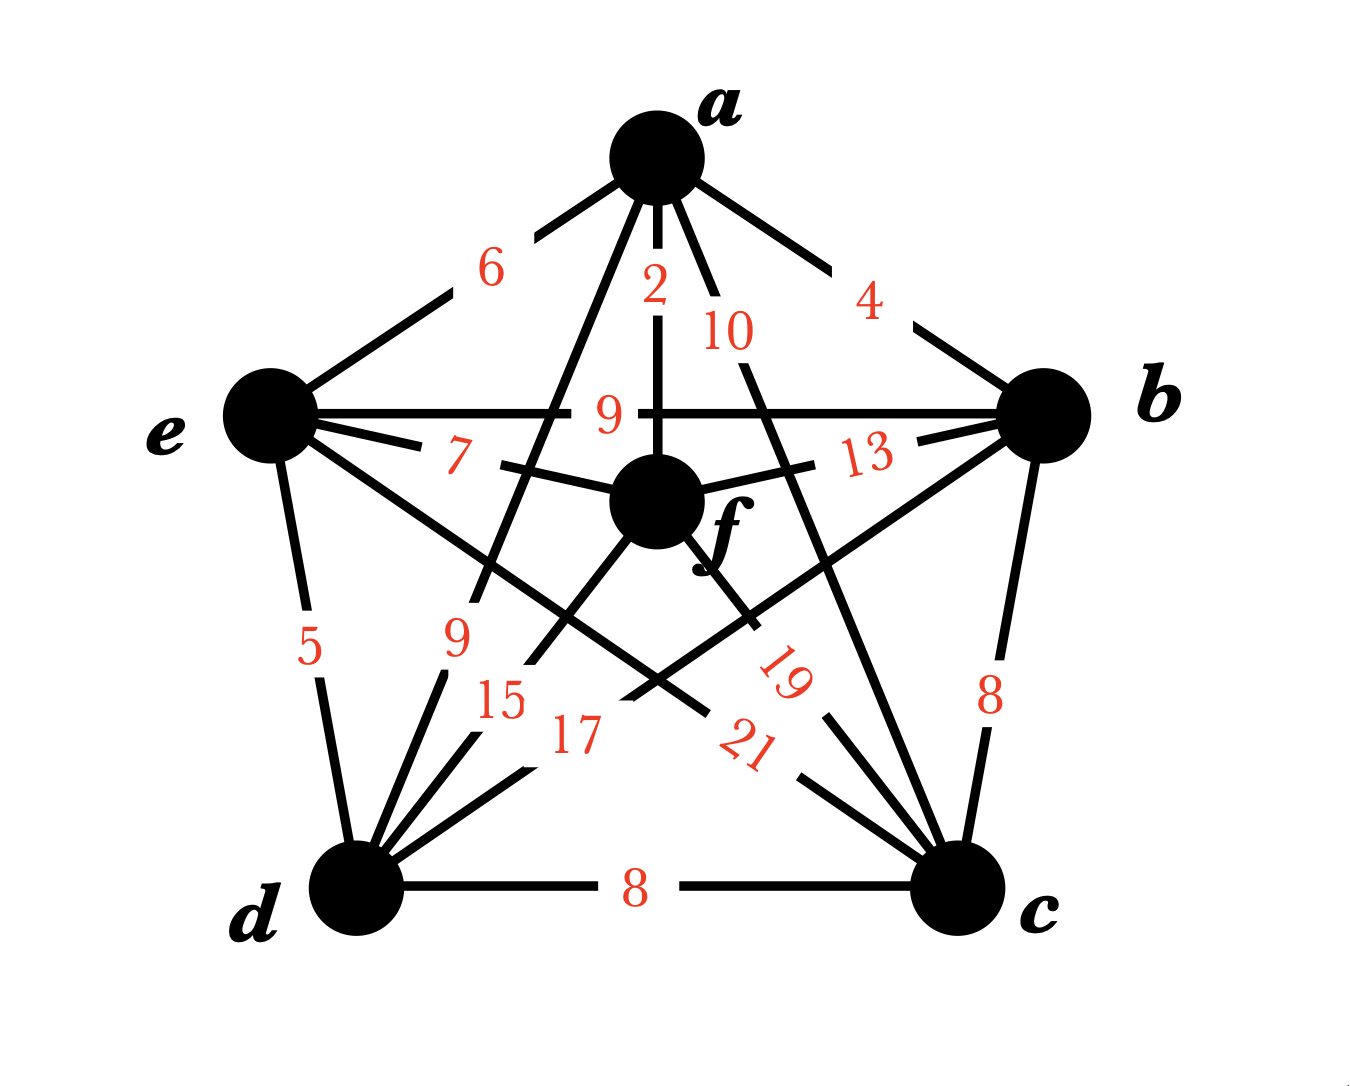
\includegraphics[width=5cm]{MWST_Example}
    \end{center}
    First, we create the following table of all the edges in $G$.
    \begin{center}
      \small
      \begin{tabular}{c|c}
        Edge & Cost \\
        \hline
        $af$ & $2$ \\
        $ab$ & $4$ \\
        $de$ & $5$ \\
        $ae$ & $6$ \\
        $ef$ & $7$ \\
        $bc$ & $8$ \\
        $cd$ & 8 \\
        $ad$ & 9\\
        $be$ & 9 \\
        $ac$ & 10 \\
        $bf$ & 13 \\
        $df$ & 15 \\
        $bd$ & 17 \\
        $cf$ & 19 \\
        $ce$ & 21
      \end{tabular}
    \end{center}
    We can read the following table describing the steps in Kruskal's algorithm from left to right (i.e., we check the edge of lowest weight, then we check the components, then we select our substep).
    \begin{center}
      \begin{tabular}{c|c|c}
        Edge & Components Of $T'$& Substep to be used\\
        \hline
        $af$ & $\{a\},\{b\},\{c\},\{d\},\{e\},\{f\}$ & 2.1 \\
        $ab$ & $\{a,f\},\{b\},\{c\},\{d\},\{e\}$ & 2.1 \\
        $de$ & $\{a,b,f\},\{c\},\{d\},\{e\}$ & 2.1 \\
        $ae$ & $\{a,b,f\},\{c\},\{d,e\}$ & 2.1 \\
        $ef$ & $\{a,b,d,e,f\},\{c\}$ & 2.2 \\
        $bc$ & $\{a,b,d,e,f\},\{c\}$ & 2.1 \\
        --- & $\{a,b,c,d,e,f\}$ & ---
      \end{tabular}
    \end{center}
  \end{problem}
  \begin{problem}{Proof of Kruskal's Algorithm}
    If $G$ is connected, then Kruskal's Algorithm produces a minimum weight spanning tree.
    \tcblower
    Let $G$ be a connected graph, and let $T_K$ be the output from Kruskal's algorithm on $G$. It is easy to check that $T_K$ is a spanning tree, since it is acyclic and has $n(G) - 1$ edges.\\

    Suppose $T^*$ is a MWST with largest edge intersection with $T_K$ --- in other words, $|E(T_K)\cap E(T^*)| \geq |E(T_K)\cap E(T')|$ for any other MWST $T'$.\\

    If $T^* = T_K$, then we are done, since $T_K$ is assumed to be a minimum weight spanning tree. Otherwise, assume toward contradiction that $T^*\neq T_K$. Let $e$ be the first edge chosen by Kruskal's algorithm that is not in $T^*$. Then, by a previous result, $\exists e'\in E(T^*) - E(T_K)$ such that $T' = T^* +e-e'$ is a spanning tree.\\

    We are assuming, however, that Kruskal's algorithm would choose $e$ over $e'$. Let $e_1,\dots,e_k$ be edges in $E(T_K)$ before $e$. Since $e_i$ was selected before $e$, we know that $e_i\in E(T^*)$ for each $i\in [k]$.\\

    Let $G_k = (V,\{e_1,\dots,e_k\})$. we are assuming that Kruskal's algorithm would not choose $e'$ for two reasons:
    \begin{itemize}
      \item If $e'$ shows up before $e$, then $e'$ would connect two vertices in $G_j = (V,\{e_1,\dots,e_j\})$. Since $G_j + e'\subseteq T^*$, then $T^*$ contains a cycle and isn't a spanning tree.
      \item If $e'$ shows up after $e$ in $L_E$, then $w(e') \geq w(e)$, meaning $w(T') \leq w(T^*)$, meaning that $w(T_K) \leq w(T^*)$, implying that $T_K$ is of a lower weight than $T^*$. 
    \end{itemize}
  \end{problem}
  \begin{problem}{Dijkstra's Algorithm}
    We want to find an algorithm to find the shortest path between two vertices in a weighted graph --- Dijkstra's Algorithm can solve this.\\

    We know that if $P$ is the shortest $u,v$ path, and $x\in P$, then following $P$ from $u$ to $x$ will yield the shortest $u,x$ path.
    \begin{description}[font=\normalfont\scshape]
      \item[Input] A weighted graph, $G$, and $u\in V(G)$
      \item[Output] For each $z\in V(G)$, the distance $d(u,z)$.
      \item[Initialization]Extend the weight function such that if $xy\notin E(G)$, then $w(xy) = \infty$. Create $S$ that contains all vertices whose distances from $u$ are known. Let $S := \{u\}$. Let $t:V\rightarrow \mathbb{R}^+ \cup \{0,\infty\}$ which will keep track of the tentative distance between $u$ and $z$. Let $t(z) := w(uz)$ for all $z\neq u$, and $t(u) := 0$.
      \item[Condition to Terminate Loop] If $t(z) = \infty$ for all $z\notin S$ \textsc{or} $S = V$, then go to end.
      \item[Loop] Else, pick $v\in V-S$ such that $t(v) = \min_{z\notin S} t(z)$. Add $v$ to $S$. Explore the edges from $v$ to update tentative distances; for each edge $vz$ with $z\notin S$, $t(z) := \min\{t(z),t(v) + w(vz)\}$.
      \item[End] Set $d(u,v) = t(v)~\forall v\in V$.
    \end{description}
    On the following weighted graph, we can do Dijkstra's algorithm as follows:
    \begin{center}
      \begin{tikzpicture}
        \filldraw (-2,0) circle (2pt)
                  (-1,1) circle (2pt)
                  (-1,-1) circle (2pt)
                  (2,0) circle (2pt)
                  (1,-1) circle (2pt)
                  (1,1) circle (2pt);
        \node[anchor = east] (u) at (-2,0) {$u$};
        \node[anchor = south east] (a) at (-1,1) {$a$};
        \node[anchor = north east] (b) at (-1,-1) {$b$};
        \node[anchor = west] (e) at (2,0) {$e$};
        \node[anchor = north west] (c) at (1,-1) {$c$};
        \node[anchor = south west] (d) at (1,1) {$d$};
        \draw (-2,0) -- node[middleweight]{\small 1} (-1,1) -- node[middleweight]{\small 1}(1,1) -- node[middleweight]{\small 2}(2,0);
        \draw (-2,0) --node[middleweight]{\small 3}(-1,-1) --node[middleweight]{\small 5} (1,-1) -- node[middleweight]{\small 6} (2,0);
        \draw (-1,-1) --node[earlyweight]{\small 4}(1,1);
        \draw (-1,1) --node[earlyweight]{\small 4}(1,-1);
      \end{tikzpicture}
    \end{center}
  \end{problem}
  \begin{problem}{Dijkstra's Algorithm: Worked Example}
    We let $S = \{u\}$, and include our tentative distances for the first step.
    \begin{center}
      \begin{tikzpicture}
        \filldraw (-2,0) circle (2pt)
                  (-1,1) circle (2pt)
                  (-1,-1) circle (2pt)
                  (2,0) circle (2pt)
                  (1,-1) circle (2pt)
                  (1,1) circle (2pt);
        \node[anchor = east] (u) at (-2,0) {\small $t_u=0$};
        \node[anchor = south east] (a) at (-1,1) {\small $t_a = 1$};
        \node[anchor = north east] (b) at (-1,-1) {\small $t_b = 3$};
        \node[anchor = west] (e) at (2,0) {\small $t_e = \infty$};
        \node[anchor = north west] (c) at (1,-1) {\small $t_d = \infty$};
        \node[anchor = south west] (d) at (1,1) {\small $t_c = \infty$};
        \draw (-2,0) -- node[middleweight]{\small 1} (-1,1) -- node[middleweight]{\small 1}(1,1) -- node[middleweight]{\small 2}(2,0);
        \draw (-2,0) --node[middleweight]{\small 3}(-1,-1) --node[middleweight]{\small 5} (1,-1) -- node[middleweight]{\small 6} (2,0);
        \draw (-1,-1) --node[earlyweight]{\small 4}(1,1);
        \draw (-1,1) --node[earlyweight]{\small 4}(1,-1);
      \end{tikzpicture}
    \end{center}
    Now, $S = \{u,a\}$ because $t_a \leq t_b$. We now start from $a$ and include our tentative distances.
    \begin{center}
      \begin{tikzpicture}
        \filldraw (-2,0) circle (2pt)
                  (-1,1) circle (2pt)
                  (-1,-1) circle (2pt)
                  (2,0) circle (2pt)
                  (1,-1) circle (2pt)
                  (1,1) circle (2pt);
        \node[anchor = east] (u) at (-2,0) {\small $t_u=0$};
        \node[anchor = south east] (a) at (-1,1) {\small $t_a = 1$};
        \node[anchor = north east] (b) at (-1,-1) {\small $t_b = 3$};
        \node[anchor = west] (e) at (2,0) {\small $t_e = \infty$};
        \node[anchor = north west] (c) at (1,-1) {\small $t_c = 5$};
        \node[anchor = south west] (d) at (1,1) {\small $t_d = 6$};
        \draw (-2,0) -- node[middleweight]{\small 1} (-1,1) -- node[middleweight]{\small 1}(1,1) -- node[middleweight]{\small 2}(2,0);
        \draw (-2,0) --node[middleweight]{\small 3}(-1,-1) --node[middleweight]{\small 5} (1,-1) -- node[middleweight]{\small 6} (2,0);
        \draw (-1,-1) --node[earlyweight]{\small 4}(1,1);
        \draw (-1,1) --node[earlyweight]{\small 4}(1,-1);
      \end{tikzpicture}
    \end{center}
    Next, we include $b$ into $S$, making it $\{u,a,b\}$. We then check our tentative distances from $b$, where we find that they are no better than tentative distances from $a$, so we keep the tentative distances on $c$ and $d$ as what they were with $a$.
    \begin{center}
      \begin{tikzpicture}
        \filldraw (-2,0) circle (2pt)
                  (-1,1) circle (2pt)
                  (-1,-1) circle (2pt)
                  (2,0) circle (2pt)
                  (1,-1) circle (2pt)
                  (1,1) circle (2pt);
        \node[anchor = east] (u) at (-2,0) {\small $t_u=0$};
        \node[anchor = south east] (a) at (-1,1) {\small $t_a = 1$};
        \node[anchor = north east] (b) at (-1,-1) {\small $t_b = 3$};
        \node[anchor = west] (e) at (2,0) {\small $t_e = \infty$};
        \node[anchor = north west] (c) at (1,-1) {\small $t_c =5$};
        \node[anchor = south west] (d) at (1,1) {\small $t_d = 6$};
        \draw (-2,0) -- node[middleweight]{\small 1} (-1,1) -- node[middleweight]{\small 1}(1,1) -- node[middleweight]{\small 2}(2,0);
        \draw (-2,0) --node[middleweight]{\small 3}(-1,-1) --node[middleweight]{\small 5} (1,-1) -- node[middleweight]{\small 6} (2,0);
        \draw (-1,-1) --node[earlyweight]{\small 4}(1,1);
        \draw (-1,1) --node[earlyweight]{\small 4}(1,-1);
      \end{tikzpicture}
    \end{center}
    Next, we include $c$ into $S$, making it $\{u,a,b,c\}$, and we update our tentative distances.
    \begin{center}
      \begin{tikzpicture}
        \filldraw (-2,0) circle (2pt)
                  (-1,1) circle (2pt)
                  (-1,-1) circle (2pt)
                  (2,0) circle (2pt)
                  (1,-1) circle (2pt)
                  (1,1) circle (2pt);
        \node[anchor = east] (u) at (-2,0) {\small $t_u=0$};
        \node[anchor = south east] (a) at (-1,1) {\small $t_a = 1$};
        \node[anchor = north east] (b) at (-1,-1) {\small $t_b = 3$};
        \node[anchor = west] (e) at (2,0) {\small $t_e = 11$};
        \node[anchor = north west] (c) at (1,-1) {\small $t_c =5$};
        \node[anchor = south west] (d) at (1,1) {\small $t_d = 6$};
        \draw (-2,0) -- node[middleweight]{\small 1} (-1,1) -- node[middleweight]{\small 1}(1,1) -- node[middleweight]{\small 2}(2,0);
        \draw (-2,0) --node[middleweight]{\small 3}(-1,-1) --node[middleweight]{\small 5} (1,-1) -- node[middleweight]{\small 6} (2,0);
        \draw (-1,-1) --node[earlyweight]{\small 4}(1,1);
        \draw (-1,1) --node[earlyweight]{\small 4}(1,-1);
      \end{tikzpicture}
    \end{center}
    Finally, we include $d$ and update tentative distances:
    \begin{center}
      \begin{tikzpicture}
        \filldraw (-2,0) circle (2pt)
                  (-1,1) circle (2pt)
                  (-1,-1) circle (2pt)
                  (2,0) circle (2pt)
                  (1,-1) circle (2pt)
                  (1,1) circle (2pt);
        \node[anchor = east] (u) at (-2,0) {\small $t_u=0$};
        \node[anchor = south east] (a) at (-1,1) {\small $t_a = 1$};
        \node[anchor = north east] (b) at (-1,-1) {\small $t_b = 3$};
        \node[anchor = west] (e) at (2,0) {\small $t_e = 8$};
        \node[anchor = north west] (c) at (1,-1) {\small $t_c =5$};
        \node[anchor = south west] (d) at (1,1) {\small $t_d = 6$};
        \draw (-2,0) -- node[middleweight]{\small 1} (-1,1) -- node[middleweight]{\small 1}(1,1) -- node[middleweight]{\small 2}(2,0);
        \draw (-2,0) --node[middleweight]{\small 3}(-1,-1) --node[middleweight]{\small 5} (1,-1) -- node[middleweight]{\small 6} (2,0);
        \draw (-1,-1) --node[earlyweight]{\small 4}(1,1);
        \draw (-1,1) --node[earlyweight]{\small 4}(1,-1);
      \end{tikzpicture}
    \end{center}
    In order to find the direct paths, we can add arrows along the edges that were selected by Dijkstra's algorithm.\\

    The proof can be outlined as follows:
    \begin{description}[font=\normalfont\scshape]
      \item[If $z\in S$:] then, $t(z) = d(u,z)$.
      \item[Else if $z\notin S$:] then, $t(z)$ is the length of a shortest $u,z$ path $P$ such that $V(P-z)\subseteq S$.
    \end{description}
  \end{problem}
  \section*{3.1}%
  \begin{problem}{Matchings}
    In a simple graph, a \textbf{matching} $M$ is a set of pairwise disjoint edges. In other words, $\forall e_i,e_j\in M$, then $e_i\cap e_j = \emptyset$. In an arbitrary graph, a matching is a set of non-loop edges with no shared endpoints. For example, the thick edges are a matching.
    \begin{center}
      \begin{tikzpicture}
        \filldraw (1,1) circle (2pt)
              (1,-1) circle (2pt)
              (-1,1) circle (2pt)
              (-1,-1) circle (2pt);
        \draw (1,1) -- (1,-1) -- (-1,-1) -- (-1,1)-- cycle;
        \draw[very thick] (1,1) -- (-1,-1);
        \draw[very thick] (-1,1) -- (1,-1);
      \end{tikzpicture}
    \end{center}
    If $v$ is incident to an edge, then $v$ is \textbf{saturated} by $M$, otherwise it is unsatured by $M$.\\

    A \textbf{perfect matching} is a matching that saturates every vertex. We know that all graphs with perfect matchings have even number of vertices, but the alternative case may not be true (for example, we might consider a graph with an isolated vertex).\\

    A \textbf{maximal matching} is a matching that cannot be enlarged by adding any other edges. A \textbf{maximum} matching is a matching of maximum size among all matchings. In other words, if $M^*$ is a maximum matching, then $|M^*| \geq |M|~\forall M\in G$.
    \begin{itemize}
      \item Not every maximal matching is a maximum matching.
      \item However, every maximum matching is a maximal matching (because you cannot extend a maximum matching by definition).
    \end{itemize}
  \end{problem}
  \begin{problem}{Alternating and Augmenting Paths}
    Given a matching $M$, an $M$-\textbf{alternating path} is a path that alternates between edges in $M$ and edges not in $M$. An $M$-alternating path whose endpoints are unsaturated by $M$ is an $M$-\textbf{augmenting} path.
    \begin{center}
      An $M$-alternating path: \\
      \vspace{10pt}
      \begin{tikzpicture}
        \filldraw (-2,0) circle (2pt)
                  (-1,1) circle (2pt)
                  (0,0) circle (2pt)
                  (1,1) circle (2pt)
                  (2,0) circle (2pt);
        \draw (-2,0) -- (-1,1);
        \draw[very thick] (-1,1) -- (0,0);
        \draw (0,0) -- (1,1);
        \draw[very thick] (1,1) -- (2,0);
      \end{tikzpicture}\\
      \vspace{20pt}
      An $M$-augmenting path:\\
      \vspace{10pt}
      \begin{tikzpicture}
        \filldraw (-2,0) circle (2pt)
                  (-1,1) circle (2pt)
                  (0,0) circle (2pt)
                  (1,1) circle (2pt)
                  (2,0) circle (2pt)
                  (3,1) circle (2pt);
        \draw (-2,0) -- (-1,1);
        \draw[very thick] (-1,1) -- (0,0);
        \draw (0,0) -- (1,1);
        \draw[very thick] (1,1) -- (2,0);
        \draw (2,0) -- (3,1);
      \end{tikzpicture}
    \end{center}
    If $M$ is a matching and there exists an $M$-augmenting path in $G$, then $M$ is not a maximum matching (as in the path $P$ that contains $M$, you can switch the matching edges as follows)
    \begin{center}
      \begin{tikzpicture}
        \filldraw (-2,0) circle (2pt)
                  (-1,1) circle (2pt)
                  (0,0) circle (2pt)
                  (1,1) circle (2pt)
                  (2,0) circle (2pt)
                  (3,1) circle (2pt);
        \draw[very thick] (-2,0) -- (-1,1);
        \draw (-1,1) -- (0,0);
        \draw[very thick](0,0) -- (1,1);
        \draw (1,1) -- (2,0);
        \draw[very thick] (2,0) -- (3,1);
      \end{tikzpicture}
    \end{center}
  \end{problem}
  \begin{problem}{Symmetric Difference}
    The \textbf{symmetric difference} $G\vartriangle H$ is the subgraph of $G\cup H$ whose edges are the edges of $G\cup H$ that appear in exactly one of $G$ and $H$. A picture of an example of a symmetric difference between matchings is shown below.
    \begin{center}
      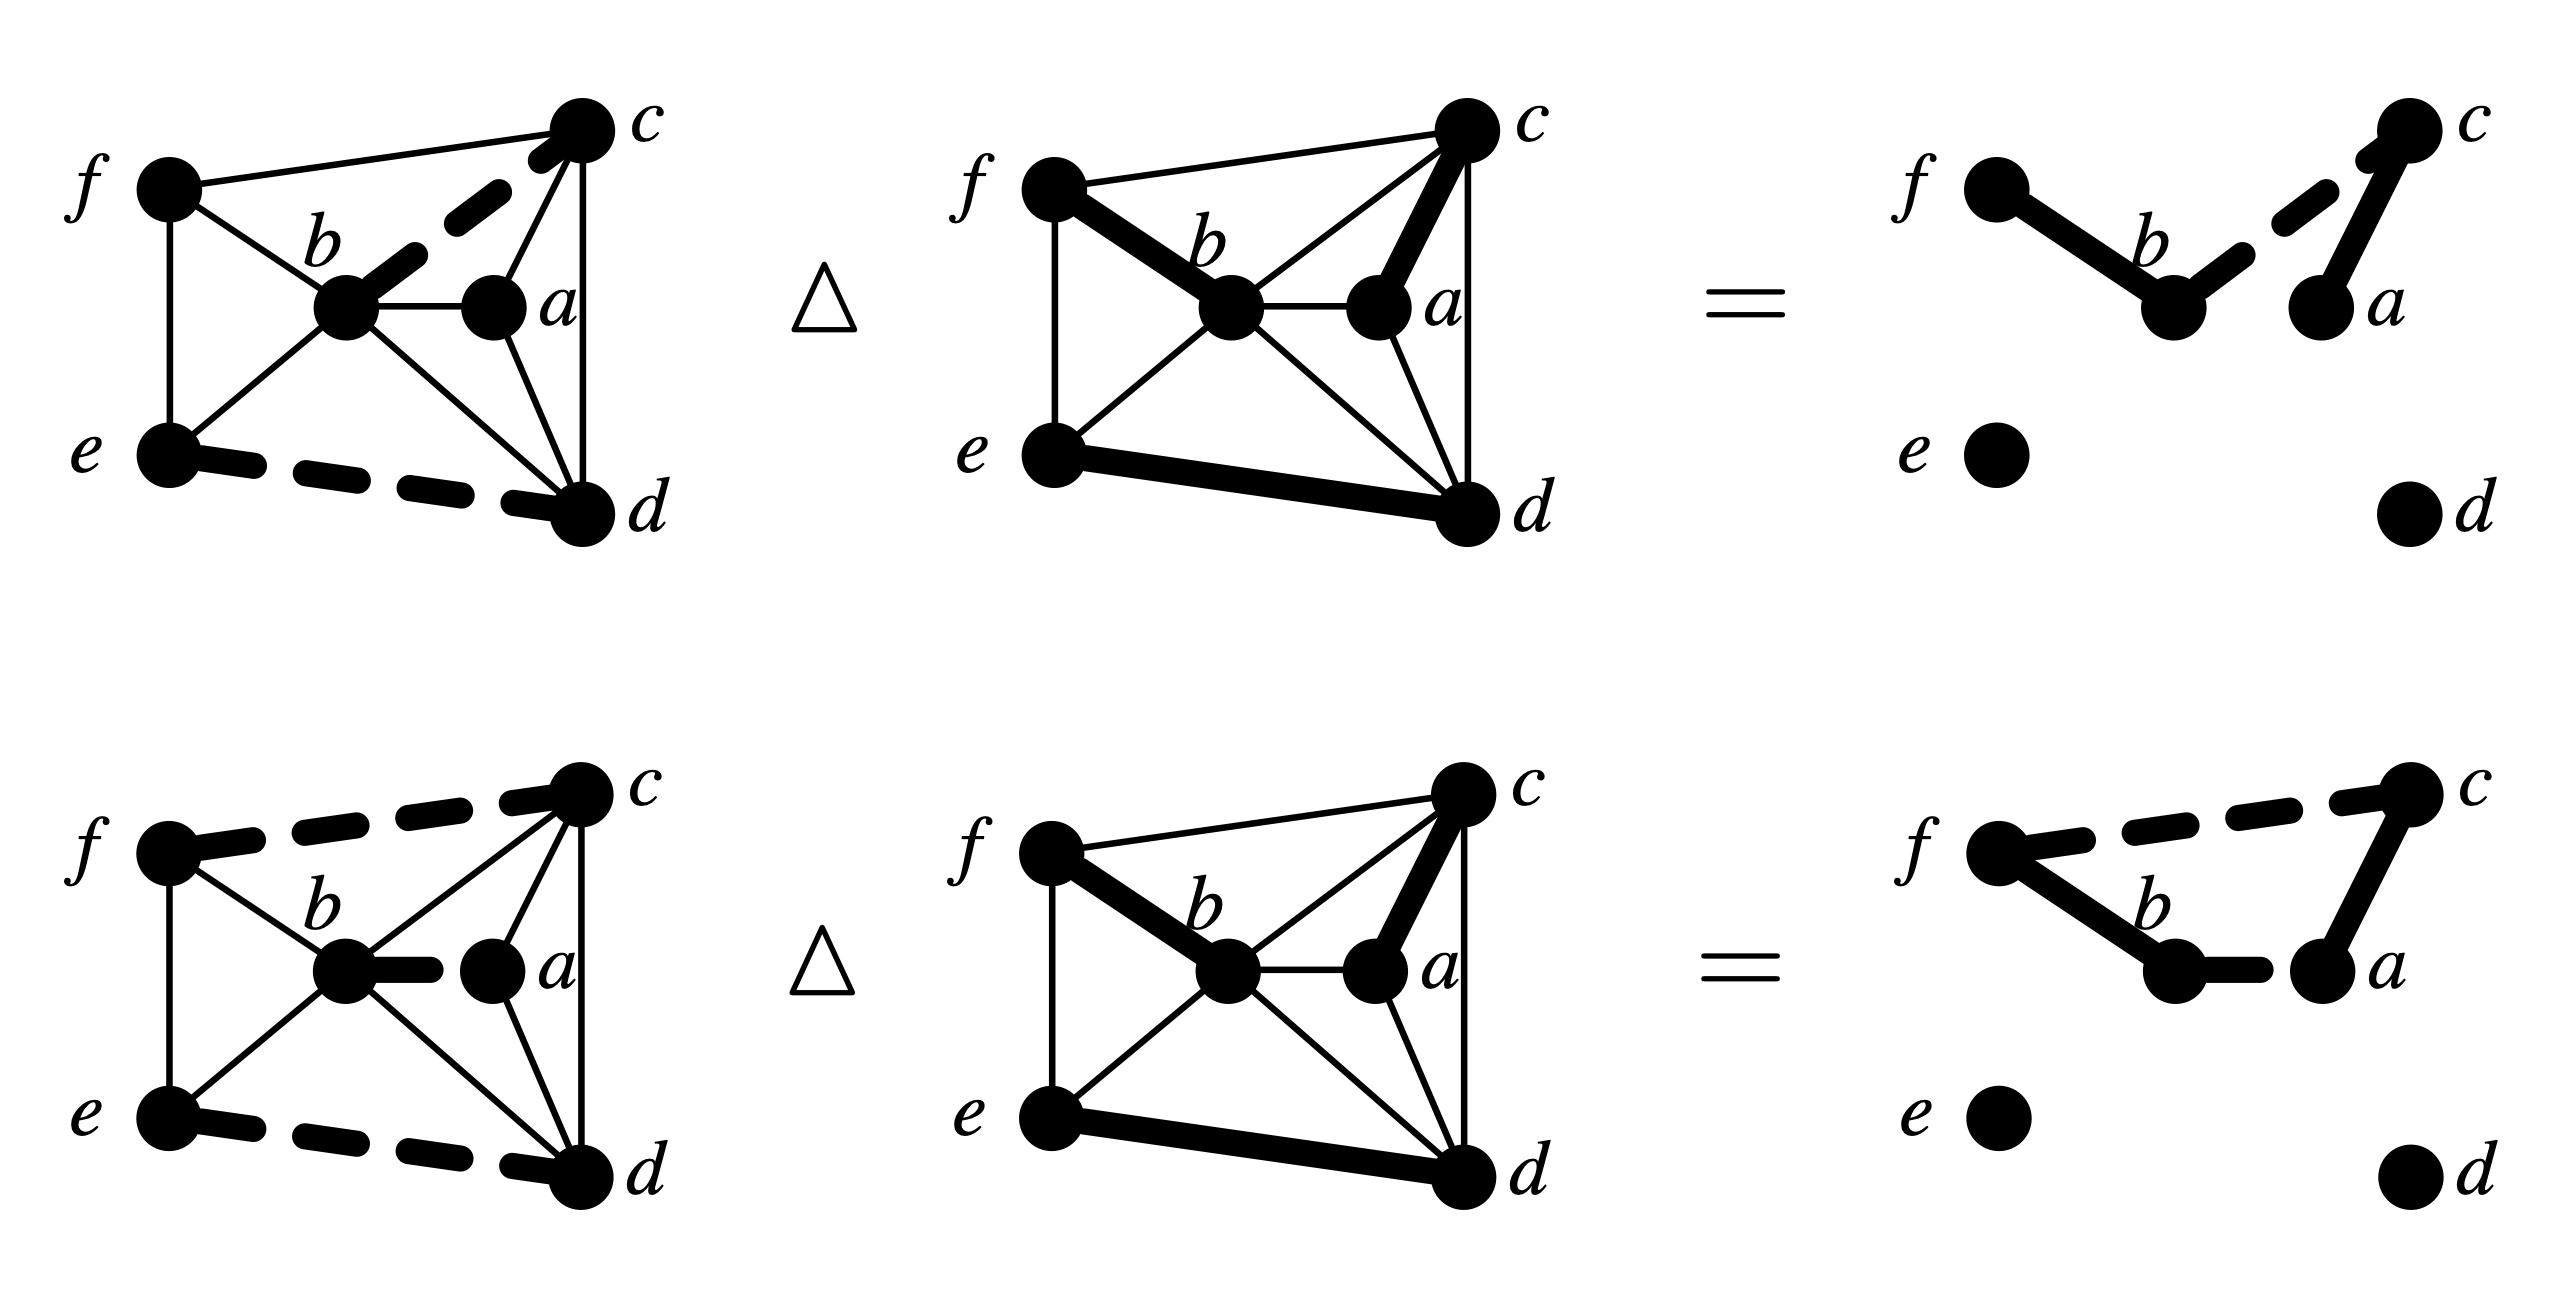
\includegraphics[width=12cm]{symmetric_difference}
    \end{center}
  \end{problem}
  \begin{problem}{Theorems and Lemmas}
    \begin{problem}{Lemma 3.1.9}
      Every component of the symmetric difference of two matchings is a path or an even cycle.
      \tcblower
      Let $M$ and $M'$ be two matchings. Each vertex is incident to at most $1$ edge in $M$ and at most one edge in $M'$. Thus, $d(v)\leq 2$ for each vertex in $M$ and $M'$. Therefore, each component is either a path or a cycle.\\

      If a component is a cycle, then it must be even because the edges of the cycle must alternate between $M$ and $M'$.
    \end{problem}
    \begin{problem}{Theorem 3.1.10}
      A matching $M$ in a graph $G$ is a \textit{maximum} matching if and only if $G$ has no $M$-augmenting path.
      \tcblower
      \begin{description}[font=\normalfont\scshape]
        \item[($\Rightarrow$)] Suppose $G$ has an $M$-augmenting path, $P$. Exchange the edges of $P$ in $M$ with the edges of $P$ not in $M$. This action increases the size of the matching by $1$, meaning that $M$ was not a maximum matching initially.
        \item[$\Leftarrow$] Suppose $M$ is not a maximum matching. Let $M'$ be a matching with more edges than $M$ (i.e., $|M'| > |M|$). Let $H = (V(G),M\vartriangle M')$. By Lemma 3.1.9, we know that each component of $H$ is either a path or an even cycle. Since $|M'| > |M|$, there is a component of $H$ that contains more edges from $M'$ than edges from $M$, which means it cannot be an even cycle --- therefore, this component must be a path that alternates between $M'$ and $M$. Because there are more edges from $M'$ than $M$ in this path, meaning this path is an $M$-augmenting path.
      \end{description}
    \end{problem}
  \end{problem}
  \begin{problem}{Perfect Matchings}
    Let $G = (X,E,Y)$ be a bipartite graph. A matching that saturates $X$ is an $X$-\textbf{perfect matching}.\\

    If there exists a set of vertices $S\subseteq X$ such that $|S| > |N(S)|$, then it is impossible for $G$ to have an $X$-perfect matching.
    \begin{problem}{Theorem 3.1.11 (Hall, 1935)}
      A bipartite graph $G = (X,E,Y)$ has an $X$-perfect matching if and only if $|S| \leq |N(S)|$ for all $S\subseteq X$.
      \tcblower
      \begin{description}[font=\normalfont\scshape]
        \item[($\Rightarrow$)] If $G$ has an $X$-perfect matching, then each vertex in $X$ is matched to a distinct vertex in $N(S)$. Thus, $|S| \leq |N(S)|$.
        \item[($\Leftarrow$)] We will prove via the contrapositive. Suppose $G$ does not have an $X$-perfect matching. Let $M$ be a maximum matching in $G$, and let $u\in X$ be an $M$-unsaturated vertex. Let $S = \{x\in X: \exists~M\textrm{-alternating $u,x$ path}\}$, and $T = \{y\in Y: \exists M\textrm{-alternating $u,y$ path}\}$.\\

          We can partition $S$ into $\{u\},X_1,\dots,X_k$ and $T$ into $Y_1,\dots,Y_k$, where $|X_i| = |Y_i|$ for $1\leq i\leq k$. Our partition works as follows: $Y_1 = N(u), X_1 = N_M(Y_1), Y_2 = N(X_1)-Y_1, X_2 = N_M(Y_2)$, and the general form is $Y_i = N(X_{i-1}) - (Y_1\cup \cdots \cup Y_{i-1})$ and $X_i = N_M(Y_i)$.\\

          Since $M$ is a maximum matching, we know that there are no $M$-augmenting paths, meaning $|X_i| = |Y_i|$ (otherwise, if $|X_i| < |Y_i|$, we would be able to find a $M$-augmenting $u,y$ path). Therefore, $|S| = |\{u\}| + |X_1| + \cdots + |X_k|$ while $|T| = |Y_1| + \cdots + |Y_k|$, so $|S| = |T| + 1$.
      \end{description}
    \end{problem}
    \begin{problem}{Corollary 3.1.13}
      For $k>0$, every $k$-regular bipartite graph has a perfect matching.
      \tcblower
      Let $k>0$ and let $G = (X,E,Y)$ be a $k$-regular bipartite graph. We will show that $G$ satisfies Hall's condition. Let $S\subseteq X$ and $[S,N(S)] = \{xy\in E(G): x\in S \textrm{ and } y\in N(S)\}$, and $[X,N(S)] = \{xy\in E(G): x\in X \textrm{ and } y\in N(S)\}$. Since $[S,N(S)] \subseteq [X,N(S)]$. Additionally, $\sum_{x\in S} d(X) = |[S,N(S)]|$ and $\sum_{y\in X}d(y) = |[X,N(S)]|$.\\

      Since $G$ is $k$=regular, we find that $|[S,N(S)]| = k|S|$ and $|[X,N(S)]| = k|N(S)|$, meaning that $|S| \leq |N(S)|$
    \end{problem}
  \end{problem}
  \begin{problem}{Vertex Covers}
    A \textbf{vertex cover} is a set $Q\subseteq V(G)$ such that $Q$ contains at least one endpoint of every edge. A picture of two vertex covers is shown below:
    \begin{center}
      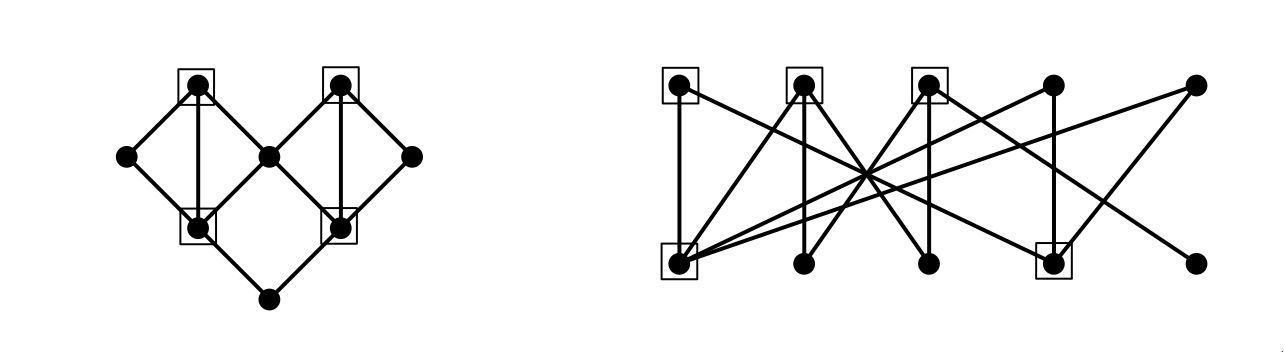
\includegraphics[width=10cm]{vertex_covers}
    \end{center}
    Of course, a very simple way to find a vertex cover is to select every vertex into $Q$. However, that isn't particularly useful, so we are focused on \textit{small} vertex covers.\\
    \begin{itemize}
      \item The size of the \textbf{minimum vertex cover} is $\beta(G)$.
      \item The size of the \textbf{maximum matching} is $\alpha'(G)$ (the edge correspondent to $\alpha(G)$ for the size of the maximum independent set).
    \end{itemize}
    Alternatively, the minimum vertex cover is denoted $\tau(G)$ and the maximum matching is denoted $\nu(G)$.\\
    
    An example of minimum vertex covers is shown below:
    \begin{center}
      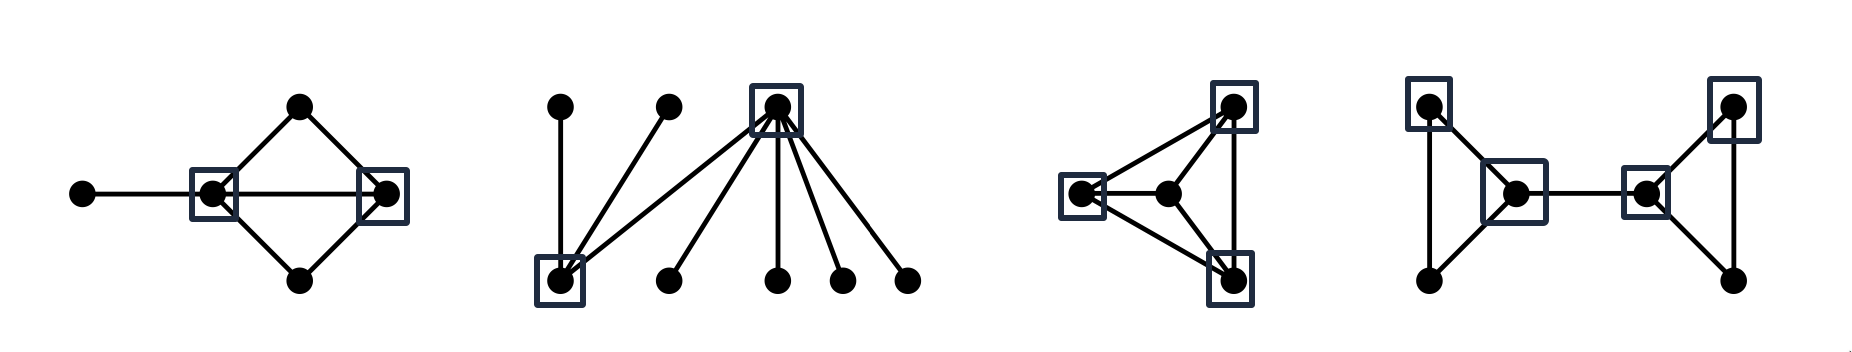
\includegraphics[width=10cm]{vertex_cover_example}
    \end{center}
    For any graph $G$, we can see that $\alpha'(G) \leq \beta(G)$ because to cover the edge of the maximum matching, we will need at least one vertex per edge in the maximum matching. Therefore, the minimum vertex cover must contain within it every vertex corresponding to an edge in the maximum matching, so $\beta(G) \geq \alpha'(G)$.\\

    \begin{problem}{Theorem 3.1.16 (König-Egervary Theorem)}
      If $G$ is a bipartite graph, then $\beta(G) = \alpha'(G)$.
      \tcblower
      Let $G=(X,E,Y)$ be a bipartite graph, and let $M$ be a maximum matching in $G$. We are going to show that there exists a $Q$ such that $|Q|=|M|$.\\

      For each $e$ in $M$, with endpoints $x\in X$ and $y\in Y$, select either $x$ or $y$ to be in $Q$ as follows:
      \begin{description}[font = \normalfont\scshape]
        \item[Rule:] If there exists an $M$-alternating path that starts at an unsaturated vertex $u\in X$ and ends at $y$, then $y\in Q$ --- else, $x\in Q$.
        \item[Claim:] $Q$ is a vertex cover. We will use cases to show that every edge has at least one endpoint in $Q$. 
          \begin{description}[font = \normalfont\scshape]
            \item[Case 1:] Suppose $xy\in M$. Then, $x\in Q\veebar y\in Q$.
            \item[Case 2:] Suppose $xy\notin M$. If $x$ is $M$-unsaturated, then $y$ must be $M$-saturated (or else we would add the edge to the matching). We can create an $M$-alternating path that starts at $x$ and ends at $y$, meaning that $y\in Q$.\\

              Otherwise, if $x$ is $M$-saturated, let $xv\in M$ --- then, we can find that $v\in Q$ because we create an $M$-alternating path that starts at $u\in X$ and ends at $v$. If $P$ does not contain $y$, then we extend by going from $v$ to $x$ to $y$.
          \end{description}
      \end{description}
    \end{problem}
  \end{problem}
  \begin{problem}{Edge Covers}
    An \textbf{edge cover} is a set of edges $A$ such that every vertex is incident to some edge in $A$. If $A$ is an edge cover, then $\bigcup_{e\in A} e = V(G)$.\\

    The \textbf{edge cover number} is the size of a minimum edge cover of $G$. It is denoted $\beta'(G)$.\\

    We can see a relationship between vertex covers and independent sets as follows, where the top graph shows the minimum vertex cover and the bottom graph shows the maximum independent set.
    \begin{center}
      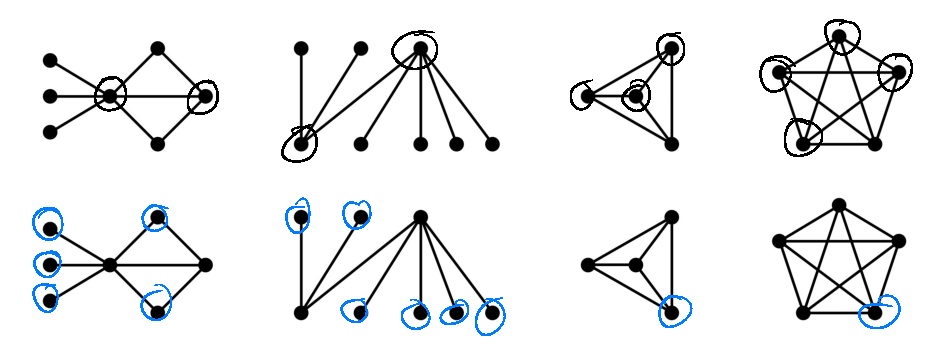
\includegraphics[width=10cm]{vertex-cover-independent-set}
    \end{center}
    Similarly, we can see a relationship between minimum edge covers and maximum matchings.
    \begin{center}
      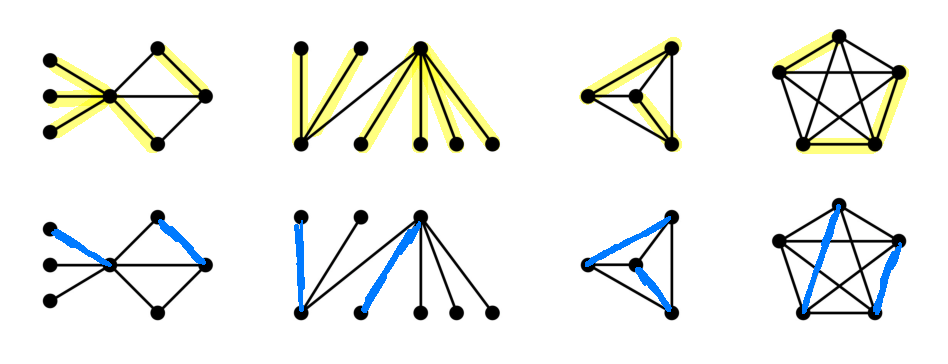
\includegraphics[width=10cm]{edge-cover-maximum-matching}
    \end{center}
  \end{problem}
  \begin{problem}{Theorems and Lemmas}
    Following from the previous result regarding independent sets and vertex covers, we might be able to state the following propostions:
    \begin{problem}{Lemma 3.1.21}
      In a graph $G$, $S\subseteq V(G)$ is an independent set if and only if $\overline{S}$ is a vertex cover. Therefore, we get the following result:
      \[
        \alpha(G) + \beta(G) = n(G)
      \] 
      \tcblower
      \begin{description}
        \item[] $S$ is an independent set.
        \item[$\Leftrightarrow$] $\forall u,v\in S, u\not\leftrightarrow v$.
        \item[$\Leftrightarrow$] $\forall e\in e(G)$, both endpoints of $e$ are not in $S$.
        \item[$\Leftrightarrow$] Both endpoints of $e$ are in $\overline{S}$.
        \item[$\Leftrightarrow$] $\overline{S}$ is a vertex cover.
      \end{description}
      Thus, if $S$ is a maximum independent set, then $\overline{S}$ is a minimum vertex cover, and since $|S| + |\overline{S}| = n(G)$, this means $\alpha(G) + \beta(G) = S$.
    \end{problem}
    \begin{problem}{Theorem 3.1.22 (Gallai's Theorem)}
      If $G$ is a graph without isolated vertices, then $\alpha'(G) + \beta'(G) = n(G)$. (i.e., if $G$ is a graph without isolated vertices, then the size of a minimum edge cover summed with the size of the maximum matching equals the number of vertices in $G$).
      \tcblower
      We will prove the forward direction first, as follows:\\

      Let $M$ be a maximum matching, and let $A = V(M)$ and $B = \overline{A}$. Since $M$ is a maximum matching, $\not\exists e\in E(G)$ such that $e$ connects two edges in $B$ (or else you could simply add it to the matching). Additionally, since there are no isolated vertices in $G$, $\forall v\in B, \exists w\in A$ such that $v\leftrightarrow w$. \\

      Select one edge such that $e = vw$ for each $v\in B$, and let the set of these edges be $N$. Then, $C = M\cup N$ is an edge cover, as every vertex in $A$ is covered by $M$, and every vertex in $B$ is covered by $N$. So, we have the following:
      \begin{align*}
        |M| + |C| &= |M| + (|M| + |N|) \tag*{Since $M$ and $N$ are disjoint}\\
            &= \left(\frac{|A|}{2}\right) + \left(\frac{|A|}{2} + |B|\right) \tag*{By the definition of $M$ and $N$}\\
            &= n(G)
      \end{align*}
      So, we have that $|M| + |C| = n(G) \geq \alpha'(G) + \beta'(G)$.\\

      \vspace{10pt}
      Now, we will prove the reverse direction:\\
      
      Let $C$ be a minimum edge cover. The components of $C$ are stars (there are no cycles or copies of $P_4$). Let $M$ be a matching formed by taking one edge from each edge in each component of $C$. Assign each ``center'' vertex in with an edge from $M$ and assign each ``leaf'' edge with an edge from $C$.\\

      Each vertex in $V(G)$ appears exactly once in each star, we have that $n(G) = |M| + |C|$. So, since $|C| = \beta'(G)$ and $|M| \leq \alpha'(G)$, we have that $|M| + |C| = n(G) \leq \alpha'(G) + \beta'(G)$.\\

      Since $n(G) \geq \alpha'(G) + \beta'(G)$ and $n(G) \leq \alpha'(G) + \beta'(G)$, we have that $n(G) = \alpha'(G) + \beta'(G)$.
    \end{problem}
    \begin{problem}{Corollary 3.1.24}
      If $G$ is a bipartite graph with no isolated vertices, then $\alpha(G) = \beta'(G)$.
      \tcblower
      We previously showed that $\alpha(G) + \beta(G) = n(G)$ and $\alpha'(G) + \beta'(G) = n(G)$, and by the König-Egerváry theorem, we know that $\alpha'(G) = \beta(G)$ in bipartite graphs with non-isolated vertices, so $\alpha(G) + \beta(G) - \beta(G) = \alpha'(G) - \alpha'(G) + \beta'(G)$, so $\alpha(G) = \beta'(G)$.
    \end{problem}
  \end{problem}
  \begin{problem}{Our Hungarian Method for Maximum Matchings}
    This is a method for finding a maximum matching in a bipartite graph that builds off the augmenting path algorithm. Consider the graph below:
    \begin{center}
      \begin{tikzpicture}
        \filldraw (0,1) circle (2pt)
                  (1,1) circle (2pt)
                  (2,1) circle (2pt)
                  (3,1) circle (2pt)
                  (4,1) circle (2pt)
                  (0,0) circle (2pt)
                  (1,0) circle (2pt)
                  (2,0) circle (2pt)
                  (3,0) circle (2pt)
                  (4,0) circle (2pt)
                  (5,0) circle (2pt);
        \draw (0,1) -- (0,0)
              (1,1) -- (0,0)
              (2,1) -- (0,0)
              (2,1) -- (2,0)
              (2,1) -- (1,0)
              (3,1) -- (1,0)
              (3,1) -- (2,0)
              (4,1) -- (2,0)
              (4,1) -- (3,0)
              (4,1) -- (4,0)
              (4,1) -- (5,0);
        \draw[very thick] (2,1) -- (0,0);
        \draw[very thick] (4,1) -- (2,0);
      \end{tikzpicture}
    \end{center}
    We will find the maximum matching by creating a ``Hungarian Forest'' as follows:
    \begin{description}[font=\normalfont\scshape]
      \item[Initialization] In our graph, we set $X_0 = \{x_1,x_2,x_4\}$ and $Y_0 = \{y_2,y_4,y_5,y_6\}$, where $X_0 \cup Y_0$ are the set of $M$-unsaturated vertices in $G$.
      \item[Iteration] Set $X_1 = X_0$ and $Y_1 = N(X_1)$. Then, we do $X_2 = N_M(X_1)$, and $Y_2 = N(X_2) - Y_1$, and so on. The general case is $X_n = N_M(Y_{n-1})$, and $Y_n = N(X_n) - Y_{n-1}$.
      \item[End condition] If $Y_n$ is empty, then we stop the algorithm.
    \end{description}
    Let $Y^* = \bigcup Y_i$ (the vertices of $Y$ that are in our Hungarian Forest). If $Y_0 \cap Y^* = \emptyset$, then $M$ is a maximum matching. Otherwise, select $y\in Y_0 \cap Y^*$, and follow the path from $y$ to the root of the tree to create an $M$-augmenting path, and ``flip'' the path (exchange matching edges with non-matching edges). In this case, after flipping the path starting between $x_4$ and $y_2$, yielding the following graph.
    \begin{center}
      \begin{tikzpicture}
        \filldraw (0,1) circle (2pt)
                  (1,1) circle (2pt)
                  (2,1) circle (2pt)
                  (3,1) circle (2pt)
                  (4,1) circle (2pt)
                  (0,0) circle (2pt)
                  (1,0) circle (2pt)
                  (2,0) circle (2pt)
                  (3,0) circle (2pt)
                  (4,0) circle (2pt)
                  (5,0) circle (2pt);
        \draw (0,1) -- (0,0)
              (1,1) -- (0,0)
              (2,1) -- (0,0)
              (2,1) -- (2,0)
              (2,1) -- (1,0)
              (3,1) -- (1,0)
              (3,1) -- (2,0)
              (4,1) -- (2,0)
              (4,1) -- (3,0)
              (4,1) -- (4,0)
              (4,1) -- (5,0);
        \draw[very thick] (2,1) -- (0,0);
        \draw[very thick] (4,1) -- (2,0);
        \draw[very thick] (3,1) -- (1,0);
      \end{tikzpicture}
    \end{center}
    After building our Hungarian forest in the same process, we find that $Y_0 \cap Y^* \neq \emptyset$, so we pick an $M$-augmenting path starting at $y_4$, and flip the path starting at $y_4$ following up to $x_1$. Afterwards, we find the graph as follows:
    \begin{center}
      \begin{tikzpicture}
        \filldraw (0,1) circle (2pt)
                  (1,1) circle (2pt)
                  (2,1) circle (2pt)
                  (3,1) circle (2pt)
                  (4,1) circle (2pt)
                  (0,0) circle (2pt)
                  (1,0) circle (2pt)
                  (2,0) circle (2pt)
                  (3,0) circle (2pt)
                  (4,0) circle (2pt)
                  (5,0) circle (2pt);
        \draw (0,1) -- (0,0)
              (1,1) -- (0,0)
              (2,1) -- (0,0)
              (2,1) -- (2,0)
              (2,1) -- (1,0)
              (3,1) -- (1,0)
              (3,1) -- (2,0)
              (4,1) -- (2,0)
              (4,1) -- (3,0)
              (4,1) -- (4,0)
              (4,1) -- (5,0);
        \draw[very thick] (0,1) -- (0,0);
        \draw[very thick] (2,1) -- (2,0);
        \draw[very thick] (3,0) -- (4,1);
        \draw[very thick] (1,0) -- (3,1);
      \end{tikzpicture}
    \end{center}
  \end{problem}
  \section*{3.3}%
  \begin{problem}{Preliminary}
    \begin{description}
      \item[Q:] Suppose $G = (X,E,Y)$ is a bipartite graph that \textit{does not} have a $X$-perfect matching. What does Hall's Theorem imply about $G$?
      \item[A:] There must exist a subset $A\subseteq X$ such that $|A| > |N(A)|$.
    \end{description}
    If you have a bipartite graph, you can \textit{either} find an $X$-perfect matching, or you can find $A\subseteq X$ such that $|A| > |N(A)|$. We can test this proposition on the following set of bipartite graphs:
    \begin{center}
      \begin{tikzpicture}
        \node[anchor = east] at (-1,1) {$X$};
        \node[anchor = east] at (-1,0) {$Y$};
        \filldraw (0,1) circle (2pt)
                  (1,1) circle (2pt)
                  (2,1) circle (2pt)
                  (3,1) circle (2pt)
                  (1,0) circle (2pt)
                  (2,0) circle (2pt)
                  (3,0) circle (2pt)
                  (4,0) circle (2pt);
        \draw (0,1) -- (1,0);
        \draw (1,1) -- (1,0);
        \draw (1,1) -- (2,0);
        \draw (2,1) -- (1,0);
        \draw (2,1) -- (2,0);
        \draw (3,1) -- (2,0);
        \draw (3,1) -- (3,0);
        \draw (3,1) -- (4,0);
        \draw (0,1) circle (4pt);
        \draw (1,1) circle (4pt);
        \draw (2,1) circle (4pt);
      \end{tikzpicture}
    \end{center}
    In the above graph, we can see that there is a set of vertices $X$ such that the set of neighbors is of smaller cardinality.
    \begin{center}
      \begin{tikzpicture}
        \node[anchor = east] at (-1,1) {$X$};
        \node[anchor = east] at (-1,0) {$Y$};
        \filldraw (0,1) circle (2pt)
                  (1,1) circle (2pt)
                  (2,1) circle (2pt)
                  (3,1) circle (2pt)
                  (1,0) circle (2pt)
                  (2,0) circle (2pt)
                  (4,0) circle (2pt);
        \draw (0,1) -- (1,0);
        \draw (1,1) -- (2,0);
        \draw (2,1) -- (2,0);
        \draw (3,1) -- (2,0);
        \draw (3,1) -- (4,0);
        \draw (2,1) -- (1,0);
        \draw (0,1) circle (4pt)
              (1,1) circle (4pt)
              (2,1) circle (4pt)
              (3,1) circle (4pt);
      \end{tikzpicture}
    \end{center}
    In the above graph, we can see that the entirety of $X$ is of a larger cardinality than the entirety of $N(X)$, so there cannot be an $X$-perfect matching.
    \begin{center}
      \begin{tikzpicture}
        \node[anchor = east] at (-1,1) {$X$};
        \node[anchor = east] at (-1,0) {$Y$};
        \filldraw (0,1) circle (2pt)
                  (1,1) circle (2pt)
                  (2,1) circle (2pt)
                  (3,1) circle (2pt)
                  (0,0) circle (2pt)
                  (1,0) circle (2pt)
                  (2,0) circle (2pt)
                  (3,0) circle (2pt);
        \draw (0,1) -- (1,0);
        \draw (0,1) -- (2,0);
        \draw (1,1) -- (0,0);
        \draw (1,1) -- (1,0);
        \draw (1,1) -- (3,0);
        \draw (2,1) -- (1,0);
        \draw (2,1) -- (2,0);
        \draw (3,1) -- (1,0);
        \draw (3,1) -- (2,0);
        \draw (0,1) circle (4pt)
              (2,1) circle (4pt)
              (3,1) circle (4pt);
      \end{tikzpicture}
    \end{center}
    In the above graph, we can see that there is a subset of $X$ such that $N(S)$ is of smaller cardinality than $S$.
    \begin{center}
      \begin{tikzpicture}
        \node[anchor = east] at (-1,1) {$X$};
        \node[anchor = east] at (-1,0) {$Y$};
        \filldraw (0,1) circle (2pt)
                  (1,1) circle (2pt)
                  (2,1) circle (2pt)
                  (3,1) circle (2pt)
                  (1,0) circle (2pt)
                  (2,0) circle (2pt)
                  (3,0) circle (2pt)
                  (4,0) circle (2pt);
        \draw[very thick] (0,1) -- (1,0);
        \draw[very thick] (1,1) -- (2,0);
        \draw (2,1) -- (1,0);
        \draw (2,1) -- (2,0);
        \draw[very thick] (2,1) -- (4,0);
        \draw (3,1) -- (2,0);
        \draw[very thick] (3,1) -- (3,0);
        \draw (3,1) -- (4,0);
      \end{tikzpicture}
    \end{center}
    In the above graph, we have found an $X$-perfect matching.\\

    We can infer from the previous exercise that if $G = (X,E,Y)$ and $|X| = |Y|$, and $G$ does \textit{not} have a perfect matching, then we can find both $A\subseteq X$ and $B\subseteq Y$ such that $|A| > |N(A)|$ and $|B| > |N(B)|$.
  \end{problem}
  \begin{problem}{Conditions for a Perfect Matching}
    We can find a set of perfect matchings in the following graphs as follows:
    \begin{center}
      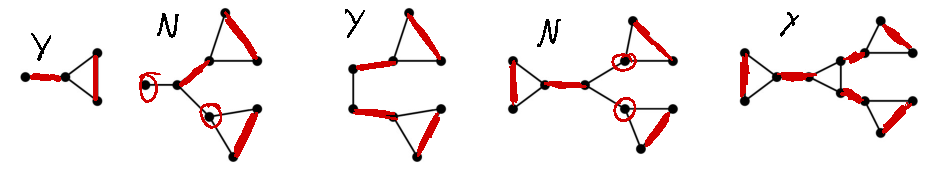
\includegraphics[width=10cm]{matchings}
    \end{center}
    From this, we can find some conditions for a perfect matching as follows:
    \begin{itemize}
      \item $n(G)$ is even
      \item For each component $H$ in $G$, $n(H)$ is even
      \item $\not\exists v\in G$ such that $G-v$ has $2$ or more odd components
    \end{itemize}
  \end{problem}
\end{document}
